\documentclass[a4paper,12pt,obeyspaces,spaces,hyphens]{article}

\def \trainingtitle{Yocto Project and OpenEmbedded development training}
\def \trainingduration{On-line seminar, 4 sessions of 4 hours}

\usepackage{agenda}

\begin{document}

\feshowtitle

\feagendasummaryitem{Title}{
  {\bf \trainingtitle{}}
}
\feagendasummaryitem{Overview}{
  Understanding the Yocto Project \par
  Using it to build a root filesystem and run it on your target \par
  Writing and extending recipes \par
  Creating layers \par
  Integrating your board in a BSP \par
  Creating custom images \par
  Application development with the Yocto Project SDK
}
\feagendasummaryitem{Materials}{
  Check that the course contents correspond to your needs:
  \newline \url{https://bootlin.com/doc/training/yocto}
}
\feagendasummaryitem{Duration}{
  {\bf Four} half days - 16 hours (4 hours per half day).
  \newline 80\% of lectures, 20\% of practical demos.
}
\feagendasummaryitem{Trainer}{
  One of the engineers listed on
  \newline \url{https://bootlin.com/training/trainers/}
}
\feagendasummaryitem{Language}{
  Oral lectures: English, French.
  \newline Materials: English.
}
\feagendasummaryitem{Audience}{
  Companies and engineers interested in using
  the Yocto Project to build their embedded Linux system.
}
\feagendasummaryitem{Prerequisites}{
  {\bf Familiarity with embedded Linux} as covered
  in our embedded Linux training
  (\url{https://bootlin.com/training/embedded-linux/}) \vspace{1em}
  \newline {\bf Familiarity with UNIX or GNU/Linux commands}
  \newline People lacking experience on this topic may get
  trained by themselves, for example with our freely available
  on-line slides:
  \url{https://bootlin.com/blog/command-line/}
}
\feagendasummaryitem{Required equipment}{
  \begin{itemize}
  \item Computer with the operating system of your choice, with the
    Google Chrome or Chromium browser for videoconferencing.
  \item Webcam and microphone (preferably from an audio headset)
  \item High speed access to the Internet
  \end{itemize}
}
\feagendasummaryitem{Materials}{
  Electronic copies of presentations,
  demo instructions and data.
}

\feagendatwocolumn
{Hardware}
{
  BeagleBone Black board
  \begin{itemize}
  \item An ARM AM335x processor from Texas Instruments (Cortex-A8
    based), 3D acceleration, etc.
  \item 512 MB of RAM
  \item 2 GB of on-board eMMC storage
        \newline(4 GB in Rev C)
  \item USB host and device
  \item HDMI output
  \item 2 x 46 pins headers, to access UARTs, SPI buses, I2C buses
    and more.
  \end{itemize}
}
{}
{
  \begin{flushright}
  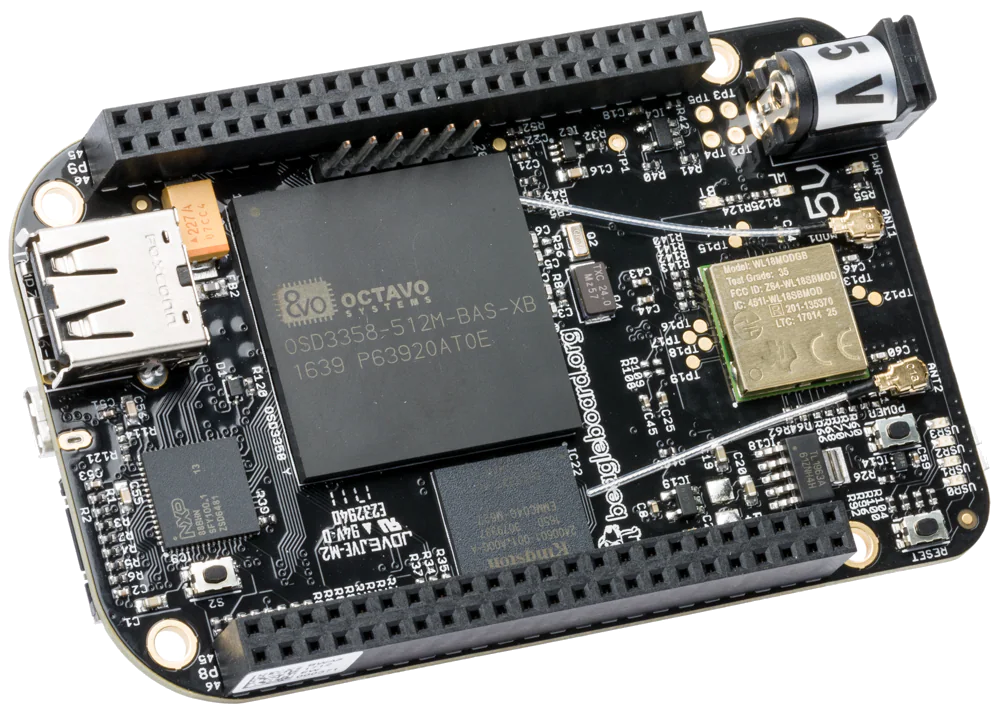
\includegraphics[width=5cm]{../slides/beagleboneblack-board/beagleboneblack.png}
  \end{flushright}
}

\section{Half day 1}

\feagendaonecolumn
{Lecture - Introduction to embedded Linux build systems}
{
  \begin{itemize}
  \item Overview of an embedded Linux system architecture
  \item Methods to build a root filesystem image
  \item Usefulness of build systems
  \end{itemize}
}
\\
\feagendatwocolumn
{Lecture - Overview of the Yocto Project and the Poky reference system}
{
  \begin{itemize}
  \item Organization of the project source tree
  \item Building a root filesystem image using the Yocto Project
  \end{itemize}
}
{Demo - First Yocto Project build}
{
  \begin{itemize}
  \item Downloading the Poky reference build system
  \item Building a system image
 \end{itemize}
}

\newpage
\feagendaonecolumn
{Lecture - Using Yocto Project - basics}
{
  \begin{itemize}
  \item Organization of the build output
  \item Flashing and installing the system image
  \end{itemize}
}

\feagendaonecolumn
{Demo - Flashing and booting}
{
  \begin{itemize}
  \item Flashing and booting the image on the board
  \end{itemize}
}

\section{Half day 2}

\feagendatwocolumn
{Lecture - Using Yocto Project - advanced usage}
{
  \begin{itemize}
  \item Configuring the build system
  \item Customizing the package selection
  \end{itemize}
}
{Demo - Using NFS and configuring the build}
{
  \begin{itemize}
  \item Configuring the board to boot over NFS
  \item Learn how to use the \code{PREFERRED_PROVIDER} mechanism
  \end{itemize}
}
\\

\feagendatwocolumn
{Lecture - Writing recipes - basics}
{
  \begin{itemize}
  \item Writing a minimal recipe
  \item Adding dependencies
  \item Development workflow with {\em bitbake}
  \end{itemize}
}
{Demo - Adding an application to the build}
{
  \begin{itemize}
  \item Writing a recipe for {\em nInvaders}
  \item Adding {\em nInvaders} to the final image
  \end{itemize}
}

\feagendaonecolumn
{Lecture - Writing recipes - advanced features}
{
  \begin{itemize}
  \item Extending and overriding recipes
  \item Adding steps to the build process
  \item Learn about classes
  \item Analysis of examples
  \item Logging
  \item Debugging dependencies
  \end{itemize}
}

\section{Half day 3}

\feagendaonecolumn
{Demo - Learning how to configure packages}
{
  \begin{itemize}
  \item Extending a recipe to add configuration files
  \item Using \code{ROOTFS_POSTPROCESS_COMMAND} to modify the final rootfs
  \item Studying package dependencies
  \end{itemize}
}

\feagendatwocolumn
{Lecture - Layers}
{
  \begin{itemize}
  \item What layers are
  \item Where to find layers
  \item Creating a layer
  \end{itemize}
}
{Demo - Writing a layer}
{
  \begin{itemize}
  \item Learn how to write a layer
  \item Add the layer to the build
  \item Move {\em nInvaders} to the new layer
  \end{itemize}
}

\feagendatwocolumn
{Lecture - Writing a BSP}
{
  \begin{itemize}
  \item Extending an existing BSP
  \item Adding a new machine
  \item Bootloaders
  \item Linux and the linux-yocto recipe
  \item Adding a custom image type
  \end{itemize}
}
{Demo - Implementing the kernel changes}
{
  \begin{itemize}
  \item Extend the kernel recipe to add the nunchuk driver
  \item Configure the kernel to compile the nunchuk driver
  \item Play {\em nInvaders}
  \end{itemize}
}

\section{Half day 4}

\feagendatwocolumn
{Lecture - Creating a custom image}
{
  \begin{itemize}
  \item Writing an image recipe
  \item Adding users/groups
  \item Adding custom configuration
  \item Writing and using package groups recipes
  \end{itemize}
}
{Demo - Creating a custom image}
{
  \begin{itemize}
  \item Writing a custom image recipe
  \item Adding {\em nInvaders} to the custom image
  \end{itemize}
}
\feagendatwocolumn
{Lecture - Creating and using an SDK}
{
  \begin{itemize}
  \item Understanding the purpose of an SDK for the application
    developer
  \item Building an SDK for the custom image
  \end{itemize}
}
{Demo - Experimenting with the SDK}
{
  \begin{itemize}
  \item Building an SDK
  \item Using the Yocto Project SDK
  \end{itemize}
}

\feagendaonecolumn
{Questions and Answers}
{
  \begin{itemize}
  \item Questions and answers with the audience about the course topics
  \item Extra presentations if time is left, according what most
        participants are interested in.
  \end{itemize}
}

\section{Possible extra time}

{\em Extra time (up to 4 hours) may be proposed if the agenda didn't fit in 4 half days,
     according to the time spent answering questions from participants.}

\end{document}

